% NeuroBench v5 — dataset overview deck
% Compile with:  latexmk -pdf neurobench_v5.tex
% (figures live in ./figures, generated by make_figures.py)

\documentclass[aspectratio=169,11pt]{beamer}

\usetheme{metropolis}
\usecolortheme{default}

\usepackage[T1]{fontenc}
\usepackage{lmodern}
\usepackage{graphicx}
\usepackage{booktabs}
\usepackage{array}
\usepackage{xcolor}
\usepackage{tikz}
\usetikzlibrary{arrows.meta, positioning, shapes.geometric}
\usepackage[most]{tcolorbox}
\usepackage{microtype}

\graphicspath{{figures/}}

\definecolor{nbgreen}{HTML}{3F6E54}
\definecolor{nbamber}{HTML}{E0A100}
\definecolor{nbred}{HTML}{B23A48}
\definecolor{nbblue}{HTML}{3D6FB5}
\definecolor{nbgrey}{HTML}{555555}

\setbeamercolor{frametitle}{bg=nbgreen,fg=white}
\setbeamercolor{title separator}{fg=nbamber}
\setbeamercolor{progress bar}{fg=nbamber,bg=nbgreen!30}
\setbeamercolor{alerted text}{fg=nbred}

\newtcolorbox{nbbox}[2][]{
  colback=nbgreen!6, colframe=nbgreen, boxrule=0.4pt,
  arc=2pt, left=4pt, right=4pt, top=3pt, bottom=3pt,
  title=#2, fonttitle=\bfseries\small, coltitle=white,
  colbacktitle=nbgreen, #1}

\newtcolorbox{redbox}[2][]{
  colback=nbred!6, colframe=nbred, boxrule=0.4pt,
  arc=2pt, left=4pt, right=4pt, top=3pt, bottom=3pt,
  title=#2, fonttitle=\bfseries\small, coltitle=white,
  colbacktitle=nbred, #1}

\newtcolorbox{bluebox}[2][]{
  colback=nbblue!6, colframe=nbblue, boxrule=0.4pt,
  arc=2pt, left=4pt, right=4pt, top=3pt, bottom=3pt,
  title=#2, fonttitle=\bfseries\small, coltitle=white,
  colbacktitle=nbblue, #1}

\title{NeuroBench v5}
\subtitle{A clinical reasoning benchmark for tool-augmented neurology agents}
\author{NeuroAgent project}
\date{\today}

\begin{document}

\maketitle

% ===================================================================
\begin{frame}{What this deck covers}
  \begin{columns}[T,onlytextwidth]
    \column{0.55\textwidth}
    \begin{itemize}\setlength\itemsep{0.45em}
      \item What NeuroBench v5 is and \alert{why we built it}
      \item How the 516 cases are generated --- the two pipelines
      \item Dataset composition: \alert{20 conditions}, difficulty, demographics
      \item The case schema and what \alert{ground truth} contains
      \item How the \alert{agent interacts} with a case (only HPI is free)
      \item A real generated patient walkthrough --- ALS-M01
    \end{itemize}

    \column{0.45\textwidth}
    \begin{nbbox}{Headline numbers}
      \begin{tabular}{@{}r l@{}}
        \textbf{516} & cases \\
        \textbf{20}  & neurological conditions \\
        \textbf{12}  & diagnostic tools \\
        \textbf{3{,}307} & pre-generated follow-up outputs \\
        \textbf{151} & cases seeded from real PMC reports \\
        \textbf{365} & fully synthetic cases \\
      \end{tabular}
    \end{nbbox}
  \end{columns}
\end{frame}

% ===================================================================
\section{What NeuroBench v5 is}

\begin{frame}{NeuroBench v5 in one slide}
  \textbf{NeuroBench v5} is a structured benchmark of \alert{516 simulated neurology
  patients} designed to evaluate tool-augmented LLM agents on clinical reasoning ---
  not on pattern recognition over a static case description.

  \vspace{0.7em}
  \begin{columns}[T,onlytextwidth]
    \column{0.5\textwidth}
    \begin{nbbox}{What's new vs.\ v1--v4}
      \begin{itemize}\setlength\itemsep{0.25em}
        \item Doubled coverage: 10 $\to$ \alert{20 conditions}
        \item Full 12-tool schema with cost tracking
        \item Difficulty rebalanced for harder cases
        \item Mix of \emph{synthetic} and \emph{real-case-seeded}
              presentations (PMC, CC-BY 4.0)
      \end{itemize}
    \end{nbbox}

    \column{0.5\textwidth}
    \begin{redbox}{What makes it a benchmark, not a quiz}
      \begin{itemize}\setlength\itemsep{0.25em}
        \item Agent only sees the \alert{initial status report} (HPI + exam + vitals)
        \item Diagnostic evidence is \alert{hidden inside tool outputs}
        \item Agent must \emph{discover} which tools to call
        \item Ground truth scores reasoning, not just final answer
      \end{itemize}
    \end{redbox}
  \end{columns}
\end{frame}

% ===================================================================
\section{How we generate cases}

\begin{frame}{Two generation pipelines}
\small
  \begin{columns}[T,onlytextwidth]
    \column{0.5\textwidth}
    \begin{bluebox}{Synthetic pipeline ($n = 365$)}
      Per-condition YAML spec describes the disease, expected tool outputs and reasoning rubric.\\[0.3em]
      LLM is given:
      \begin{enumerate}\setlength\itemsep{0.15em}
        \item Pydantic JSON schema (\texttt{NeuroBenchCase})
        \item Condition YAML
        \item Difficulty tier and encounter type
      \end{enumerate}
      Output: one JSON case validated against the schema.
    \end{bluebox}

    \column{0.5\textwidth}
    \begin{nbbox}{Real-case-seeded pipeline ($n = 151$)}
      Seed: a published PMC clinical case report (CC-BY 4.0, MedCaseReasoning corpus).\\[0.3em]
      The LLM is instructed to:
      \begin{enumerate}\setlength\itemsep{0.15em}
        \item Preserve the clinical trajectory
        \item \alert{Strip} diagnostic results out of the HPI
        \item Move them into structured \emph{tool outputs}
        \item Add red herrings at moderate/puzzle difficulty
      \end{enumerate}
    \end{nbbox}
  \end{columns}

  \vspace{0.4em}
  \begin{center}
    \small
    \textit{Both pipelines emit the same JSON schema; case IDs starting with \texttt{R} are PMC-seeded
    (e.g.\ \texttt{ALS-RS11}); the others are synthetic.}
  \end{center}
\end{frame}

% ===================================================================
\begin{frame}{The case schema --- top-level structure}
\small
  \begin{tabular}{@{}p{0.27\textwidth} p{0.69\textwidth}@{}}
    \toprule
    \textbf{Field} & \textbf{Contents} \\
    \midrule
    \texttt{case\_id}, \texttt{condition} & e.g.\ \texttt{ALS-M01}, condition enum \\
    \texttt{difficulty}                   & \emph{straightforward} / \emph{moderate} / \emph{diagnostic\_puzzle} \\
    \texttt{encounter\_type}              & \emph{outpatient} / \emph{emergency} / \emph{inpatient} \\
    \midrule
    \texttt{patient.demographics}         & age, sex, handedness, ethnicity, BMI \\
    \texttt{patient.clinical\_history}    & PMH, meds, allergies, family hx, social hx \\
    \texttt{patient.neurological\_exam}   & mental status, CNs, motor, sensory, reflexes, coord., gait \\
    \texttt{patient.vitals}               & BP, HR, T, RR, SpO\textsubscript{2} \\
    \texttt{patient.chief\_complaint}     & one-line presenting concern \\
    \texttt{patient.history\_present\_illness} & narrative HPI ($\geq$150 words) \\
    \midrule
    \texttt{initial\_tool\_outputs}       & pre-computed outputs returned on first tool call \\
    \texttt{followup\_outputs}            & conditional outputs triggered by named follow-up actions \\
    \midrule
    \texttt{ground\_truth}                & diagnosis, ICD, differential, optimal actions, critical/contraindicated actions, key reasoning, red herrings \\
    \texttt{metadata}                     & version, generation method, source PMCID/license (if seeded) \\
    \bottomrule
  \end{tabular}
\end{frame}

% ===================================================================
\section{Dataset composition}

\begin{frame}{20 conditions across neurology subspecialties}
  \begin{center}
    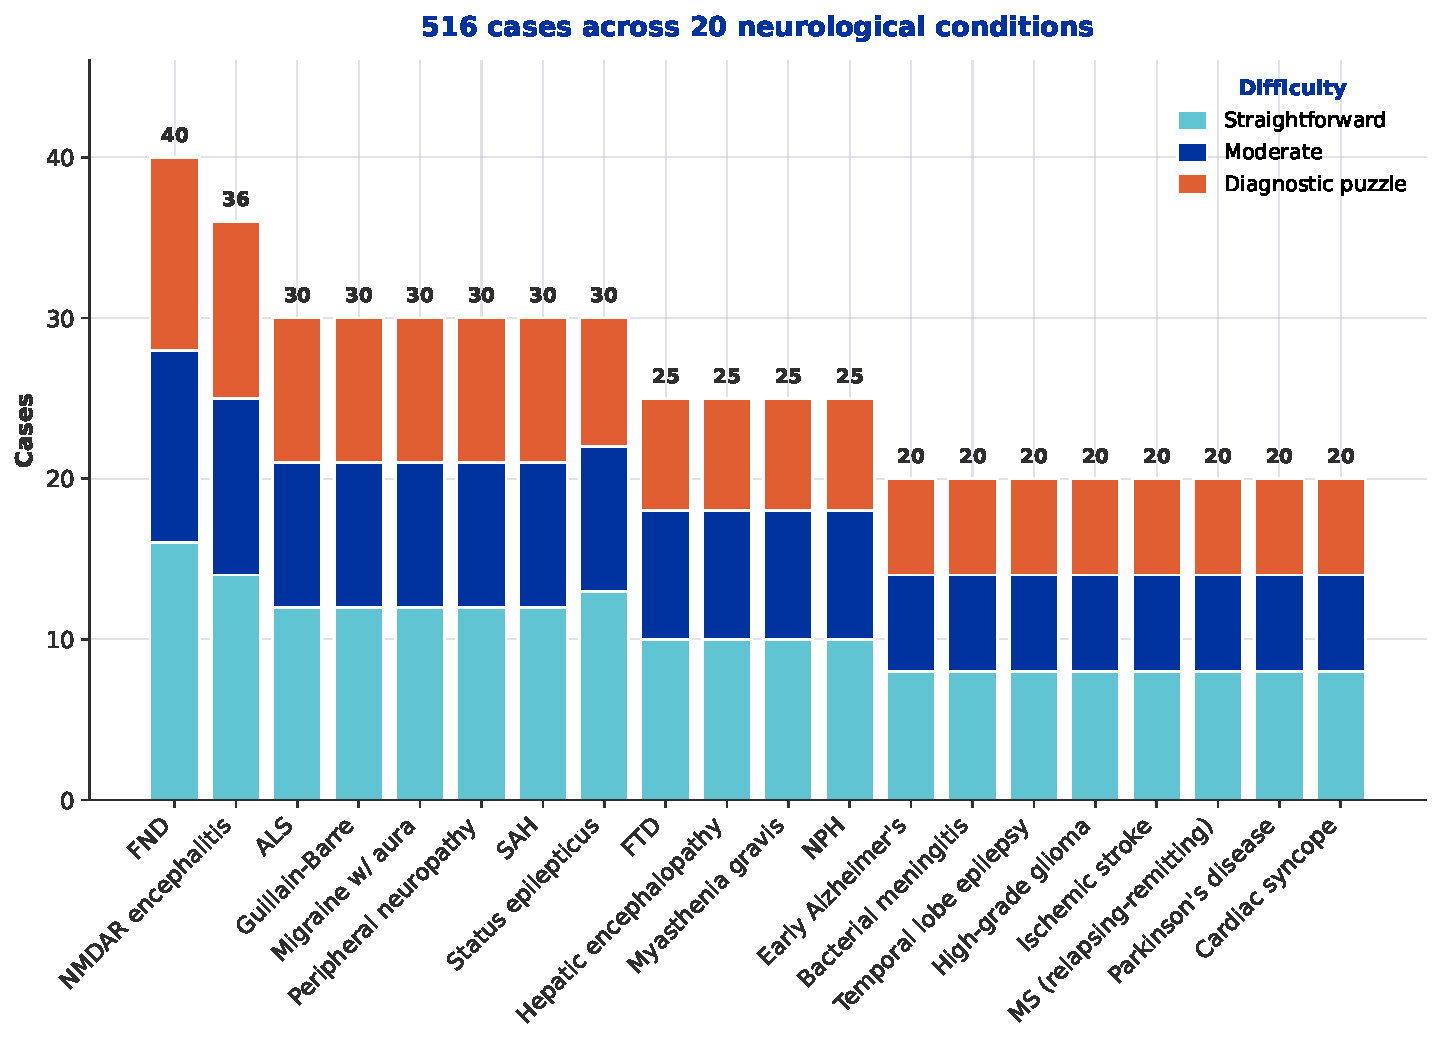
\includegraphics[width=0.96\textwidth]{condition_distribution.pdf}
  \end{center}
  \vspace{-0.5em}
  \small
  Coverage spans \alert{neuromuscular} (ALS, MG, GBS, peripheral neuropathy), \alert{epilepsy / status} (focal temporal, SE),
  \alert{vascular} (ischemic stroke, SAH, cardiac syncope), \alert{dementia} (early AD, FTD, NPH),
  \alert{demyelinating / autoimmune} (MS-RR, NMDAR encephalitis), \alert{infectious / metabolic} (bacterial meningitis, hepatic encephalopathy),
  \alert{headache} (migraine with aura), \alert{neuro-oncology} (high-grade glioma), \alert{movement} (Parkinson's), and \alert{FND}.
\end{frame}

% ===================================================================
\begin{frame}{Difficulty calibration}
  \begin{columns}[T,onlytextwidth]
    \column{0.5\textwidth}
    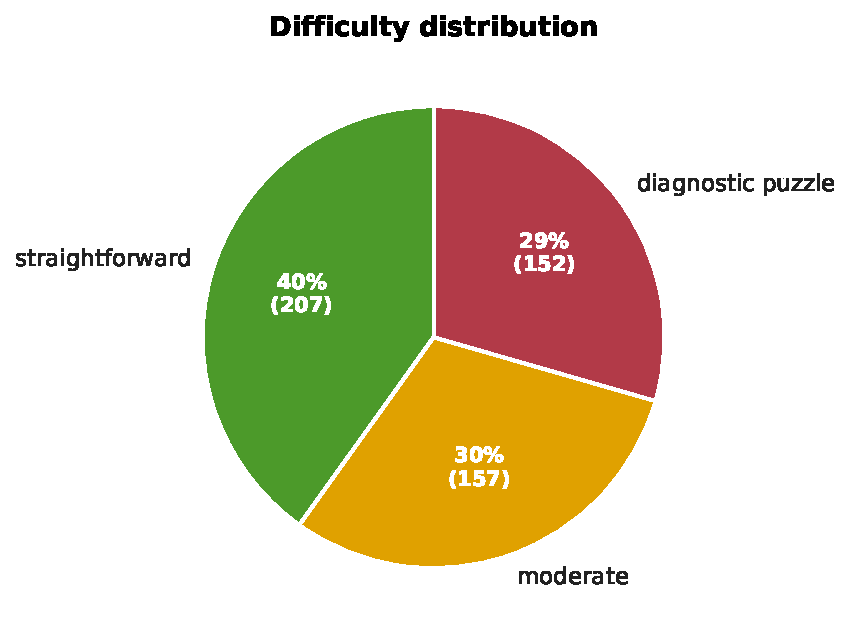
\includegraphics[width=\linewidth]{difficulty_pie.pdf}

    \column{0.5\textwidth}
    \vspace{0.4em}
    \begin{nbbox}{Straightforward (40\%)}
      Classic textbook presentation. Findings clearly point to the diagnosis. An intern should get this right.
    \end{nbbox}
    \vspace{0.2em}
    \begin{nbbox}{Moderate (30\%)}
      Atypical features or subtle findings. 1--2 \alert{red herrings} (incidental labs, borderline imaging, confounding meds).
    \end{nbbox}
    \vspace{0.2em}
    \begin{redbox}{Diagnostic puzzle (30\%)}
      Initial presentation mimics a different condition. Key diagnostic clue buried in follow-up results.
    \end{redbox}
  \end{columns}
\end{frame}

% ===================================================================
\begin{frame}{Demographics --- realistic age and sex spread}
  \begin{center}
    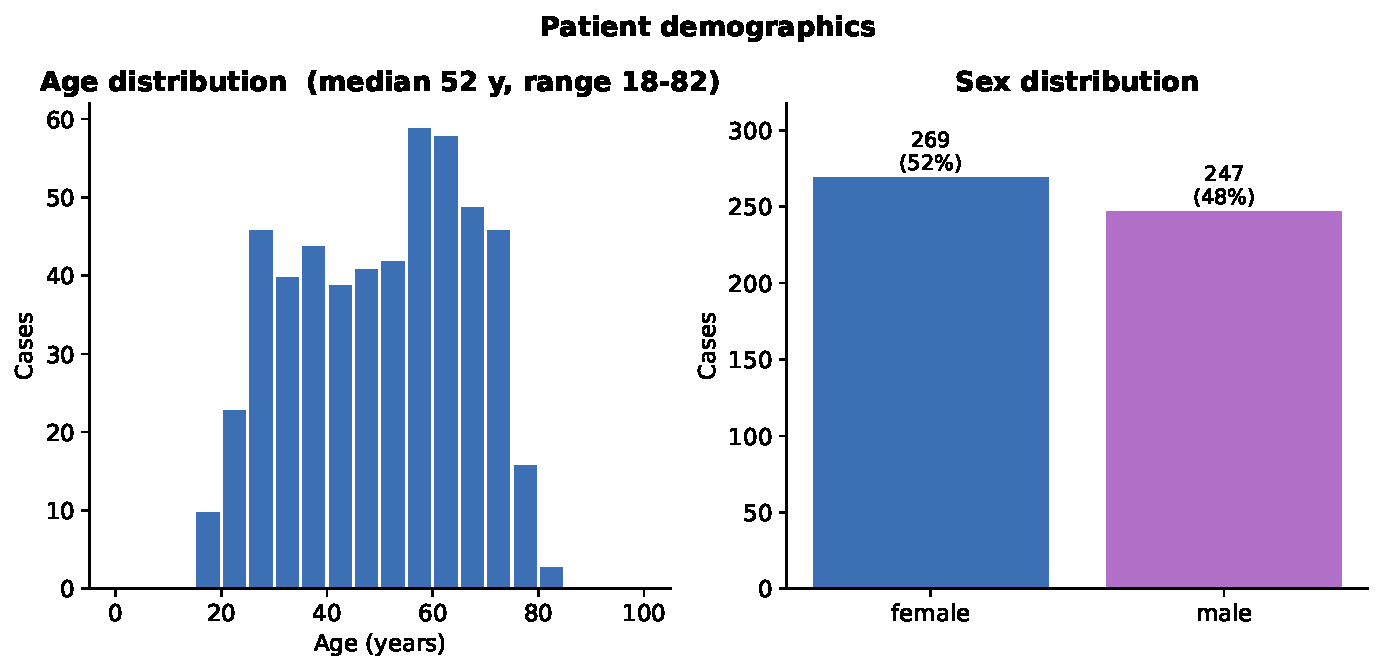
\includegraphics[width=0.96\textwidth]{demographics.pdf}
  \end{center}
  \vspace{-0.4em}
  \small
  Median age \alert{52} years, range 18--82. Sex roughly balanced (52\% female, 48\% male).
  Demographics are matched to each condition's epidemiology (e.g.\ NPH skews older, NMDAR encephalitis younger).
\end{frame}

% ===================================================================
\begin{frame}{Encounter mix and pre-generated follow-up outputs}
  \begin{center}
    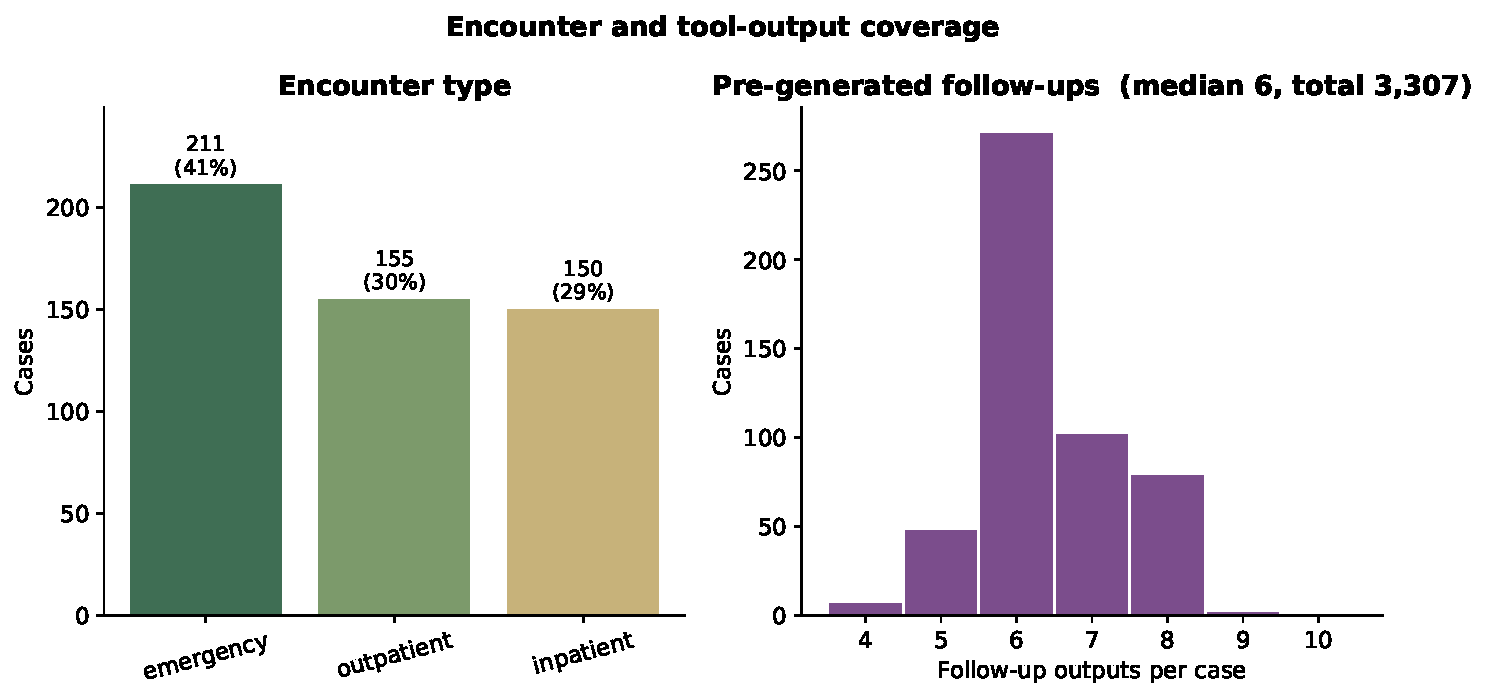
\includegraphics[width=0.96\textwidth]{encounter_and_followups.pdf}
  \end{center}
  \vspace{-0.4em}
  \small
  Each case ships with a \alert{median of 6} \texttt{followup\_outputs} keyed on \texttt{trigger\_action} ---
  e.g.\ \texttt{request\_pulmonary\_function\_als}, \texttt{check\_riluzole\_drug\_interactions}.
  Total: \alert{3{,}307} pre-cached responses across all 516 cases.
\end{frame}

% ===================================================================
\section{Tool coverage and ground truth}

\begin{frame}{The 12 diagnostic tools available to the agent}
  \begin{center}
    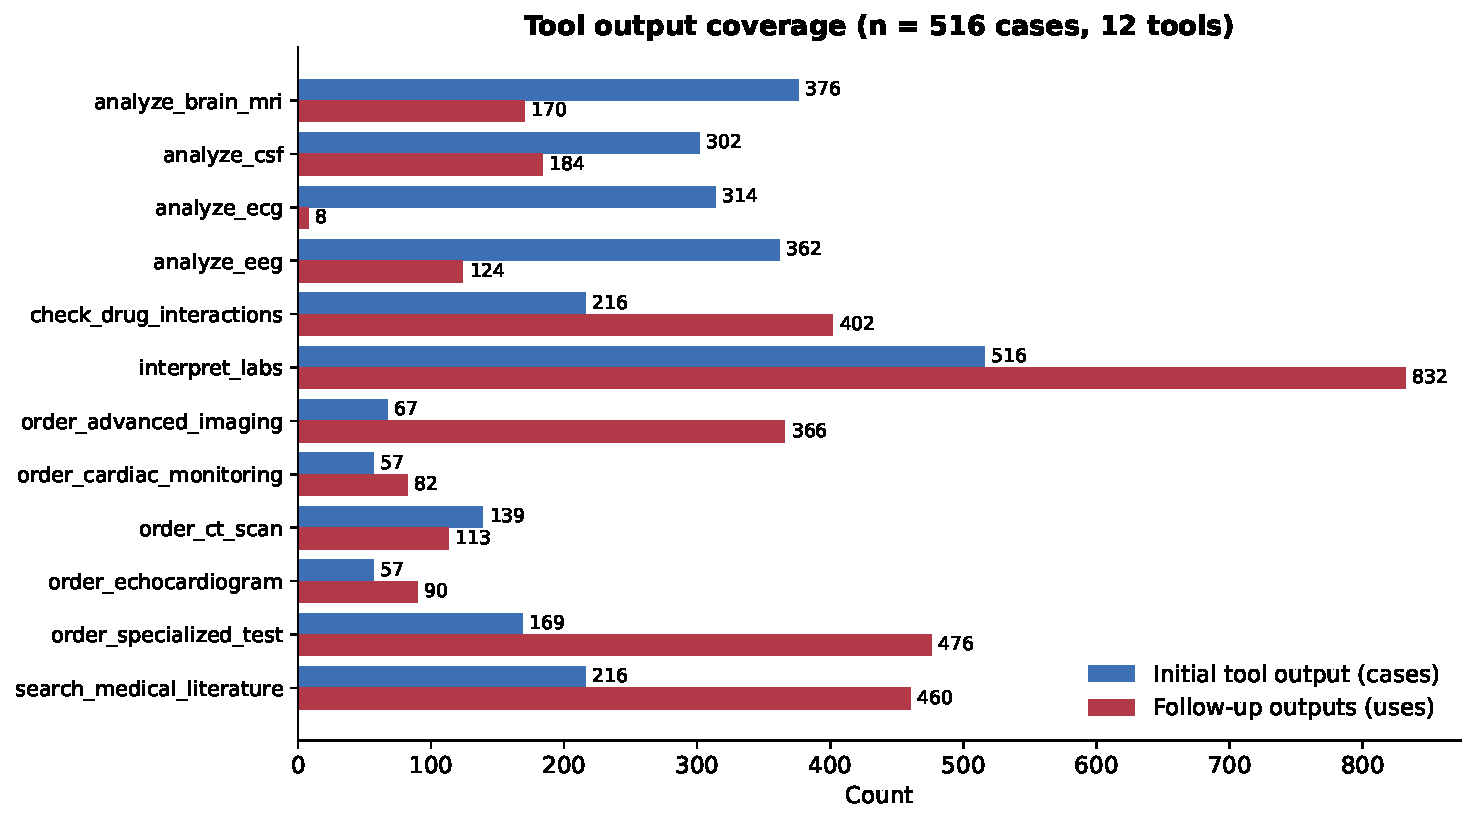
\includegraphics[width=0.88\textwidth]{tool_usage.pdf}
  \end{center}
  \vspace{-0.6em}
  \small
  \textbf{Blue:} number of cases that ship with a pre-computed initial output for that tool.\\
  \textbf{Red:} number of follow-up outputs across the dataset triggered by that tool.\\
  Every case has \texttt{interpret\_labs}; \texttt{analyze\_brain\_mri}, \texttt{analyze\_eeg}, \texttt{analyze\_ecg}, and \texttt{analyze\_csf} are present in most.
\end{frame}

% ===================================================================
\begin{frame}{Ground truth is rich --- it scores reasoning, not just answers}
  \begin{center}
    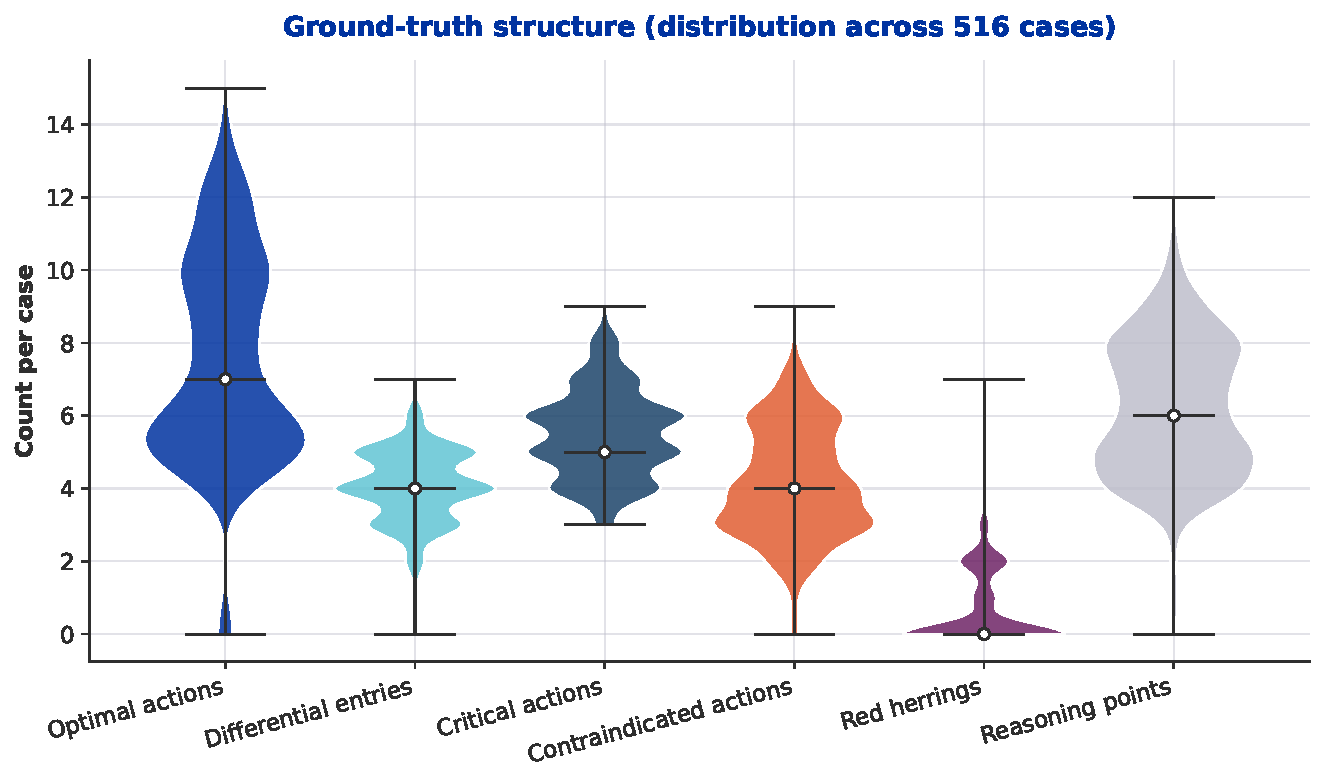
\includegraphics[width=0.88\textwidth]{groundtruth_structure.pdf}
  \end{center}
  \vspace{-0.4em}
  \small
  Each case carries a \alert{primary diagnosis} (with ICD-10), a ranked \alert{differential},
  an \alert{optimal action sequence} (each step annotated with \emph{required/acceptable}, expected finding, tool name and parameters),
  \alert{critical actions} (MUST do), \alert{contraindicated actions} (MUST NOT do),
  free-text \alert{key reasoning points}, and explicit \alert{red herrings} with the
  intended distraction and correct interpretation.
\end{frame}

% ===================================================================
\section{What the agent actually sees}

\begin{frame}{The agent does \alert{not} get everything --- it discovers}
  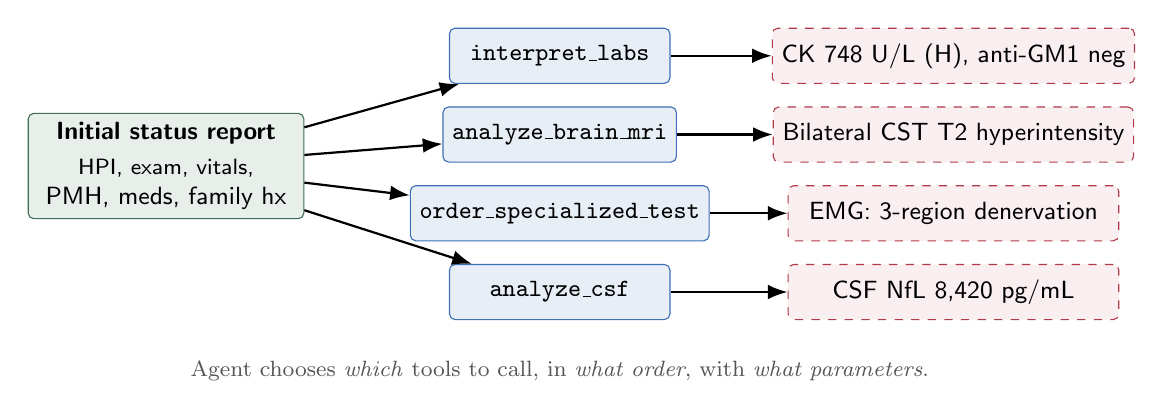
\begin{tikzpicture}[
      every node/.style={font=\small\sffamily, align=center},
      box/.style={rectangle, rounded corners=2pt, draw, minimum width=3.5cm, minimum height=1.0cm, fill=white},
      tool/.style={rectangle, rounded corners=2pt, draw=nbblue, fill=nbblue!12, minimum width=2.8cm, minimum height=0.7cm},
      ev/.style={rectangle, rounded corners=2pt, draw=nbred, dashed, fill=nbred!8, minimum width=4.2cm, minimum height=0.7cm},
      arr/.style={-{Latex[length=2.5mm]}, thick}
    ]
    \node[box, fill=nbgreen!12, draw=nbgreen] (init)
      at (0,0) {\textbf{Initial status report}\\[0.15em]
        \footnotesize HPI, exam, vitals,\\PMH, meds, family hx};

    \node[tool] (t1) at (5, 1.4) {\texttt{interpret\_labs}};
    \node[tool] (t2) at (5, 0.4) {\texttt{analyze\_brain\_mri}};
    \node[tool] (t3) at (5,-0.6) {\texttt{order\_specialized\_test}};
    \node[tool] (t4) at (5,-1.6) {\texttt{analyze\_csf}};

    \node[ev]  (e1) at (10.0, 1.4) {CK 748 U/L (H), anti-GM1 neg};
    \node[ev]  (e2) at (10.0, 0.4) {Bilateral CST T2 hyperintensity};
    \node[ev]  (e3) at (10.0,-0.6) {EMG: 3-region denervation};
    \node[ev]  (e4) at (10.0,-1.6) {CSF NfL 8{,}420 pg/mL};

    \draw[arr] (init) -- (t1);
    \draw[arr] (init) -- (t2);
    \draw[arr] (init) -- (t3);
    \draw[arr] (init) -- (t4);
    \draw[arr] (t1) -- (e1);
    \draw[arr] (t2) -- (e2);
    \draw[arr] (t3) -- (e3);
    \draw[arr] (t4) -- (e4);

    \node[font=\footnotesize, text=nbgrey] at (5,-2.6)
      {Agent chooses \emph{which} tools to call, in \emph{what order}, with \emph{what parameters}.};
  \end{tikzpicture}

  \vspace{0.6em}
  \small
  At turn 1 the agent receives a natural-language patient summary produced by
  \texttt{format\_patient\_info()}: demographics, chief complaint, narrative HPI,
  past medical history, current medications, allergies, family history, the
  full neurological exam, and vitals.

  \textbf{Crucially, none of the imaging, lab, EEG/EMG, CSF, or specialist reports are
  in that summary.} The agent has to decide what's worth ordering.
\end{frame}

% ===================================================================
\begin{frame}[fragile]{What the agent receives at turn 1 --- ALS-M01 (excerpt)}
\scriptsize
\begin{tcolorbox}[colback=black!4, colframe=black!30, boxrule=0.4pt, left=3pt, right=3pt, top=2pt, bottom=2pt]
\begin{verbatim}
Patient: 62-year-old female
Chief complaint: Progressive difficulty speaking and swallowing over 8 months,
  with bilateral arm and leg weakness
History of present illness: Ms. H is a 62-year-old right-handed woman who
  presents for neurological evaluation of an 8-month history of progressive
  dysarthria, dysphagia, and limb weakness. [...] Her primary care physician
  ordered cervical spine MRI which showed moderate spondylosis. The question
  of cervical myelopathy as the etiology of her symptoms has been raised [...]
Past medical history: Hypertension; Hypothyroidism; Osteoporosis; Remote
  right carpal tunnel syndrome, surgically released 5 years ago
Current medications: Lisinopril 10mg daily; Levothyroxine 75mcg daily; [...]
Neurological examination:
  Motor: deltoids 4/5, biceps 4+/5, intrinsic hand muscles 4-/5 R, 3+/5 L.
    Visible fasciculations in bilateral upper extremity proximal muscles.
  Reflexes: Hyperreflexia 3+ throughout. Plantar responses extensor
    bilaterally (Babinski present). Hoffman sign positive bilaterally.
  Additional: Fasciculations visible in tongue, bilateral deltoids,
    and left thenar eminence. [...]
Vitals: BP 128/78 mmHg, HR 72 bpm, Temp 36.8C, RR 14, SpO2 97%
\end{verbatim}
\end{tcolorbox}

\vspace{0.4em}
\textit{No MRI report. No labs. No EMG. No CSF. The agent must choose what to order.}
\end{frame}

% ===================================================================
\section{Case study: ALS-M01}

\begin{frame}{Case study --- ALS-M01 at a glance}
\small
  \begin{tabular}{@{}p{0.27\textwidth} p{0.69\textwidth}@{}}
    \toprule
    \textbf{Case ID}        & \texttt{ALS-M01} \\
    \textbf{Condition}      & Amyotrophic lateral sclerosis (bulbar-onset) \\
    \textbf{Difficulty}     & \alert{moderate} --- complicated by concurrent cervical spondylosis \\
    \textbf{Encounter}      & Outpatient neurology evaluation \\
    \textbf{Patient}        & 62 y female, right-handed, retired teacher, BMI 23.1 \\
    \textbf{Chief complaint} & Progressive dysarthria + dysphagia + bilateral limb weakness over 8 months \\
    \midrule
    \textbf{Ground-truth Dx} & ALS, bulbar-onset, moderate stage --- ICD-10 \alert{G12.21} \\
    \textbf{Pre-cached initial tool outputs} & MRI brain + cervical spine, comprehensive labs (incl.\ neuromuscular panel), EMG/NCS \\
    \textbf{Follow-up outputs ($n = 6$)} &
      pulmonary function, ALS genetic panel, CSF NfL, repeat EMG, ALS MDC assessment, riluzole interaction check \\
    \bottomrule
  \end{tabular}

  \vspace{0.3em}
  \begin{nbbox}{Pedagogic point}
    This case tests whether an agent will commit to neurosurgical referral for the obvious cervical
    spondylosis or recognise that bulbar findings and supra-cervical EMG denervation cannot be
    explained by cervical disease.
  \end{nbbox}
\end{frame}

% ===================================================================
\begin{frame}{ALS-M01 --- ground-truth optimal action sequence (8 steps)}
\scriptsize
  \begin{tabular}{@{}c p{0.43\textwidth} p{0.16\textwidth} p{0.27\textwidth}@{}}
    \toprule
    \# & \textbf{Action} & \textbf{Tool} & \textbf{Category} \\
    \midrule
    1 & MRI brain + cervical spine with/without contrast        & \texttt{analyze\_brain\_mri}      & required \\
    2 & Labs: CK, anti-GM1, SPEP, TSH, B12, HIV, AR-CAG repeat  & \texttt{interpret\_labs}          & required \\
    3 & EMG/NCS across bulbar, cervical, thoracic, lumbosacral  & \texttt{order\_specialized\_test} & required \\
    4 & Pulmonary function (FVC, SNIP, NIF, MIP, MEP)           & \texttt{interpret\_labs}          & required \\
    5 & ALS genetic panel (C9orf72, SOD1, TARDBP, FUS, ...)     & \texttt{interpret\_labs}          & acceptable \\
    6 & CSF neurofilament light chain (NfL) for prognosis       & \texttt{analyze\_csf}             & acceptable \\
    7 & Initiate riluzole 50 mg BID; check interactions          & \texttt{check\_drug\_interactions} & required \\
    8 & Refer to ALS multidisciplinary clinic + SLP             & ---                               & required \\
    \bottomrule
  \end{tabular}

  \vspace{0.5em}
  \small
  Each step also stores an \texttt{expected\_finding} and \texttt{tool\_parameters} block, allowing
  the evaluator to grade not just \emph{whether} the agent ordered the right test but \emph{how} it parameterised it.
\end{frame}

% ===================================================================
\begin{frame}{ALS-M01 --- differential and the two red herrings}
\small
  \begin{nbbox}{Differential as stored in the case}
    \begin{tabular}{@{}p{0.45\textwidth} p{0.16\textwidth} p{0.32\textwidth}@{}}
      \textbf{Alternative diagnosis} & \textbf{Likelihood} & \textbf{Key distinguishing feature} \\
      \midrule
      Cervical spondylotic myelopathy   & Low-mod     & Does not explain bulbar findings \\
      Multifocal motor neuropathy       & Very low    & Anti-GM1 neg, no conduction block \\
      Kennedy disease (SBMA)            & Very low    & Female sex; AR-CAG normal \\
      Progressive bulbar palsy (PBP)    & Moderate    & ALS spectrum --- EMG shows beyond bulbar \\
      Myasthenia gravis                 & Low         & No fatigability, EMG shows denervation \\
    \end{tabular}
  \end{nbbox}

  \vspace{0.5em}
  \begin{redbox}{Red herrings encoded in the case}
    \begin{itemize}\setlength\itemsep{0.15em}
      \item \textbf{Cervical spondylosis with C5--C6 stenosis} on MRI --- pulls toward neurosurgery.
            Correct interpretation: no cord-signal change; bulbar findings unexplained by cervical pathology.
      \item \textbf{Remote right CTS} surgically released 5 years ago --- suggests entrapment neuropathy as
            cause of hand weakness. Correct: EMG shows denervation in non-median muscles bilaterally.
    \end{itemize}
  \end{redbox}
\end{frame}

% ===================================================================
\begin{frame}{ALS-M01 --- what the tools actually return}
\scriptsize
  \begin{columns}[T,onlytextwidth]
    \column{0.5\textwidth}
    \begin{bluebox}{\texttt{analyze\_brain\_mri} (initial)}
      Subtle bilateral CST T2 hyperintensity in posterior limb of internal capsule.
      Multilevel cervical spondylosis, C5--C6 central stenosis, \emph{no cord signal change}.
      No demyelination, no mass, no infarct.\\
      Confidence: 0.0 --- ``clinical correlation recommended.''
    \end{bluebox}

    \vspace{0.4em}
    \begin{bluebox}{\texttt{interpret\_labs} (initial neuromuscular panel)}
      CK \textbf{748} U/L (H), Aldolase 8.2 U/L (H, mild).\\
      TSH, B12, folate, ESR, CRP normal.
      Anti-GM1 IgM negative. SPEP no M-spike. HIV non-reactive.
      AR-CAG repeat 22 (\emph{normal}).
    \end{bluebox}

    \column{0.5\textwidth}
    \begin{bluebox}{\texttt{order\_specialized\_test} (EMG/NCS, initial)}
      Active denervation + chronic reinnervation across \textbf{bulbar, cervical, thoracic};
      early lumbosacral changes. Sensory NCS \emph{normal}. No conduction block.\\
      \alert{El Escorial revised: clinically definite ALS.}
    \end{bluebox}

    \vspace{0.4em}
    \begin{bluebox}{\texttt{analyze\_csf} (follow-up after agent request)}
      OP 14 cmH\textsubscript{2}O, WBC 2 (normal), protein 58 (mildly elevated).\\
      \alert{NfL \textbf{8{,}420} pg/mL} (ref ${<}1{,}000$) --- markedly elevated.
      Oligoclonal bands absent. Cytology negative.
    \end{bluebox}
  \end{columns}

  \vspace{0.5em}
  \textit{Each output is a Pydantic model with full panel structure, reference ranges, and per-test abnormality flags.}
\end{frame}

% ===================================================================
\section{Wrap-up}

\begin{frame}{Why this design matters for the NMI paper}
  \begin{columns}[T,onlytextwidth]
    \column{0.5\textwidth}
    \begin{nbbox}{What v5 lets us measure}
      \begin{itemize}\setlength\itemsep{0.25em}
        \item \textbf{Diagnostic accuracy} on a representative slice of clinical neurology
        \item \textbf{Tool selection} --- did the agent order the right test?
        \item \textbf{Tool parameterisation} --- with the right panel/sequence/region?
        \item \textbf{Resistance to red herrings} --- did it chase the spondylosis?
        \item \textbf{Cost efficiency} --- Medicare PFS reference rates per tool call
      \end{itemize}
    \end{nbbox}

    \column{0.5\textwidth}
    \begin{redbox}{What it deliberately avoids}
      \begin{itemize}\setlength\itemsep{0.25em}
        \item \emph{Cheating via prompt}: no diagnostic findings in the initial status report
        \item \emph{Tool-call-free benchmarks}: a closed-book LLM cannot pass --- it has no labs
        \item \emph{Single-answer scoring}: ground truth grades the reasoning path
        \item \emph{Pure synthetic bias}: 30\% of cases are seeded from real PMC reports
      \end{itemize}
    \end{redbox}
  \end{columns}

  \vspace{0.4em}
  \small
  \alert{Bottom line:} an agent that calls no tools, or wrong tools, cannot succeed.
  An agent that calls the right tools and ignores their content cannot succeed either.
  We force \emph{evidence-driven} reasoning.
\end{frame}

\begin{frame}[standout]
  Thank you\\[0.4em]
  \small\normalfont 516 cases, 20 conditions, 12 tools, 3{,}307 pre-cached follow-ups, two pipelines, one schema.
\end{frame}

\end{document}
